%%%%%%%%%%%%%%%%%%%%%%%%%%%%%%%%%%%%%%%%%
% Twenty Seconds Resume/CV
% LaTeX Template
% Version 1.1 (8/1/17)
%
% This template has been downloaded from:
% http://www.LaTeXTemplates.com
%
% Original author:
% Carmine Spagnuolo (cspagnuolo@unisa.it) with major modifications by 
% Vel (vel@LaTeXTemplates.com)
%
% License:
% The MIT License (see included LICENSE file)
%
%%%%%%%%%%%%%%%%%%%%%%%%%%%%%%%%%%%%%%%%%

%----------------------------------------------------------------------------------------
%	PACKAGES AND OTHER DOCUMENT CONFIGURATIONS
%----------------------------------------------------------------------------------------

\documentclass[letterpaper]{twentysecondcv} % a4paper for A4

\usepackage[super]{nth}
\usepackage{enumitem}

\setitemize{noitemsep,topsep=0pt,parsep=0pt,partopsep=0pt}

%----------------------------------------------------------------------------------------
%	 PERSONAL INFORMATION
%----------------------------------------------------------------------------------------

\profilepic{../img/mabdelaz.jpg}

\cvname{Mostafa Abdelaziz}
\cvjobtitle{Computer and Systems Engineer}

\cvdate{30 April 1993}
\cvaddress{Metro Vancouver, Canada}
\cvnumberphone{+1 778-788-0657}
\cvsite{http://github.com/iocoder}
\cvmail{iocoder@aol.com}

%----------------------------------------------------------------------------------------

\begin{document}

%----------------------------------------------------------------------------------------
%	 ABOUT ME
%----------------------------------------------------------------------------------------

\aboutme{Professional engineer with wide technical expertise in automatic
         control systems, computer networks, computer architecture,
         embedded systems, and database systems.}

%----------------------------------------------------------------------------------------
%	 SKILLS
%----------------------------------------------------------------------------------------

\skills{
    \center{
        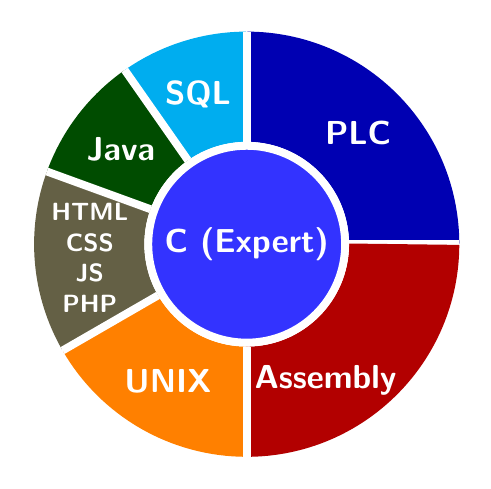
\begin{tikzpicture}[font=\sffamily\bfseries\large, text=white, border/.style={line width=14mm}]
        \foreach \angle/\col [remember=\angle as \last (initially 0)] in 
            {90/blue!70!black, 125/cyan, 160/green!30!black, 210/yellow!30!black, 270/orange, 360/red!70!black}{
                \draw[\col, border] (\last:2cm) 
                     arc[start angle=\last, end angle=\angle, radius=2cm];
                \draw[white, line width=1mm] (\last:1.3)--++(\last:1.4);
        }
        \node[line width=1mm, draw, circle, minimum width=2.5cm, white, fill=blue!80] {C (Expert)};
        \node at (45:2cm) {PLC};
        \node at (108:2cm) {SQL};
        \node at (143:2cm) {Java};
        \node[text width=1cm, align=center, font=\sffamily\bfseries\small] at (185:2cm) 
            {HTML CSS JS PHP};
        \node at (240:2cm) {UNIX};
        \node at (300:2cm) {Assembly};
        \end{tikzpicture}
    }
}

%----------------------------------------------------------------------------------------
%	 OS PREFERENCES
%----------------------------------------------------------------------------------------

\ospref{
    \textcolor{black}{
    \textbf{GNU/Linux}\hfill
\includegraphics[scale=0.40]{../img/5stars.png}\newline
    \textbf{FreeBSD}\hfill
\includegraphics[scale=0.40]{../img/4stars.png}\newline
    \textbf{Windows}\hfill
\includegraphics[scale=0.40]{../img/4stars.png}}}

%----------------------------------------------------------------------------------------
%	 LANGUAGES
%----------------------------------------------------------------------------------------

\langs{{Italian/2},{Arabic/6},{English/5.5}}

%----------------------------------------------------------------------------------------

% Print the sidebar
\makeprofile

%----------------------------------------------------------------------------------------
%	 EDUCATION
%----------------------------------------------------------------------------------------

\section{Education}

\begin{twenty} % Environment for a list with descriptions
	%\twentyitem{<dates>}{<title>}{<location>}{<description>}
	\twentyitem{2011 - 2016}
               {B.Sc., Computer and Systems Engineering}
               {Alexandria University}
               {\textbf{GPA}: 3.94.\newline
                \textbf{Overall Ranking}: \underline{\nth{1}}.\newline
                \textbf{Graduation Project}: FPGA computer based on MIPS architecture.\newline
                \textbf{Course Highlights}: Control Theory, Modern Control, Embedded Systems,
                                            Computer Architecture, Software Engineering,
                                            System Software, Operating Systems, Compilers, Switching Theory,
                                            Automata Theory, Complexity Theory.
               }
	\twentyitem{2008 - 2011}
               {High School}
               {Mubarak Secondary School, Alexandria}
               {\textbf{Overall Grade}: 407.5/410 (99.36\%).\newline
                \textbf{Specialization}: Mathematics.}
\end{twenty}

%----------------------------------------------------------------------------------------
%	 EXPERIENCE
%----------------------------------------------------------------------------------------

\section{Experience}

\begin{twenty}
	\twentyitem{Jun - Sep 17}
               {Control Systems Engineer}
               {Advanced HVAC Consultant, Cairo}
               {\underline{Role:}\newline
                PLC/DDC programming for advanced HVAC systems.
                I was the leader of a team responsible for installing and maintaining HVAC and BMS systems
                for several clients in Cairo.\newline
                \underline{Duties:}
                \begin{enumerate}
                    \item{Programming Saia Burgess PCD PLCs.}
                    \item{Designing BMS interfaces using Tridium controller.}
                    \item{Designing interfaces for various communication protocols.}
                    \item{Completing the deployment of BMS systems for several clients.}
                    \item{Instructing our teams on implementation of electrical boards.}
                    \item{Troubleshooting and solving technical problems.}
                \end{enumerate}
               }

	\twentyitem{Jul - Dec 16}
               {Software Engineer}
               {Ejada Systems Ltd., Alexandria}
               {\underline{Role:}\newline
                Programming software modules for our clients.\newline
                \underline{Duties:}
                \begin{enumerate}
                    \item Implementation of CRM systems using Oracle Siebel.
                    \item Developing BigData solutions using Hadoop and Scala.
                \end{enumerate}}

	\twentyitem{Jun - Sep 15}
               {RA Intern}
               {SmartCI Research Center, Alexandria}
               {Role: Implementation of the storage system of cognitive radio cloud.}

	%\twentyitem{<dates>}{<title>}{<location>}{<description>}
\end{twenty}

%----------------------------------------------------------------------------------------
%	 PUBLICATIONS
%----------------------------------------------------------------------------------------

\section{Selected Projects}

\begin{itemize}
    \item{Systema Programming Language.}
    \item{Quafios Operating System for x86 and MIPS.}
    \item{Radio KAOS: Cognitive Radio with Dynamic Spectrum Sharing Engine.}
    \item{CDP: Reliable Data Transfer Protocol for Linux Kernel TCP/IP Stack.}
    \item{System for OS image distribution over cloud using Frisbee.}
    \item{QCC C/Java Compiler for GNU/Linux.}
    \item{Technical Report on UEFI.}
    %\item{Liftroid: Visualized elevator interface using AVR and Android.}
    %\item{NES (Nintendo Entertainment System) Simulator.}
    %\item{IDE to USB interface using AVR and PIC.}
    %\item{8086 micro-computer system.}
    %\item{Hello World BIOS.}
    %\item{Static RAM with MOSFETs on PCB.}
    %\item{T-DEC/102, a simulated TTL computer.}
    \item{Educational Program with Animated Agent for Disabled Children.}
\end{itemize}

%----------------------------------------------------------------------------------------
%	 AWARDS
%----------------------------------------------------------------------------------------

\section{Awards}

\begin{twentyshort}
	\twentyitemshort{2017}{\textbf{IELTS} English Language Certificate, Band Score: 7.5.}
	\twentyitemshort{2017}{CSED Golden Armor for the \textbf{top student} of 2015-2016 Class.}
	\twentyitemshort{2017}{Prof. Naeem Abou Taleb Award for \textbf{top student}.}
	\twentyitemshort{2016}{\textbf{Certificate of Excellence}, Alexandria University.}
	\twentyitemshort{2015}{\textbf{Certificate of Excellence}, Alexandria University.}
	\twentyitemshort{2014}{\textbf{Certificate of Excellence}, Alexandria University.}
	\twentyitemshort{2013}{\textbf{Certificate of Excellence}, Alexandria University.}
	\twentyitemshort{2012}{Certificate of Achievement, \textbf{ACM Alexandria CPC}.}
	\twentyitemshort{2010}{Silver Medal, \textbf{Egyptian Olympiad in Informatics}.}
	\twentyitemshort{2009}{Silver Medal, \textbf{Egyptian Olympiad in Informatics}.}
	\twentyitemshort{2008}{Platinum Award, Cyberfair, \textbf{Bibliotheca Alexandrina}.}
	%\twentyitemshort{<dates>}{<title/description>}
\end{twentyshort}

\vfill
\footnotesize{
    Mailing Address: 7252 Hastings St., Burnaby, BC, Canada - V5A 1G8\newline
    You can find the \LaTeX source code of my resume at \color{blue}{http://www.github.com/iocoder/resume}.
}

\end{document} 
